
Publications in 2006}
\vspace{0.00mm}

\vspace{0.00mm}
\setlength{\parindent}{-6.25mm}
\setlength{\leftskip}{6.25mm}
\setlength{\rightskip}{-1.13mm}

\textbf{}
\vspace{0.00mm}

\vspace{0.00mm}
\setlength{\parindent}{-7.40mm}
\setlength{\leftskip}{7.40mm}
\setlength{\rightskip}{0.00mm}

\uline{Peer-reviewed Journals}

\vspace{0.00mm}

\vspace{0.00mm}
\setlength{\parindent}{0.00mm}
\setlength{\leftskip}{0.00mm}
\setlength{\rightskip}{0.00mm}

Includes: 1 Post-doc position
\vspace{0.00mm}

\vspace{0.00mm}
\setlength{\parindent}{0.00mm}
\setlength{\leftskip}{0.00mm}
\setlength{\rightskip}{0.00mm}


\vspace{0.00mm}

\vspace{0.00mm}
\setlength{\parindent}{0.00mm}
\setlength{\leftskip}{0.00mm}
\setlength{\rightskip}{0.00mm}

DAAD/PROBRAL exchange program with Brazil
\vspace{0.00mm}

\vspace{0.00mm}
\setlength{\parindent}{0.00mm}
\setlength{\leftskip}{0.00mm}
\setlength{\rightskip}{0.00mm}

\quotedblbase{}Speciation of elements of clinical and environmental relevance in saline fluids``
\vspace{0.00mm}

\vspace{0.00mm}
\setlength{\parindent}{0.00mm}
\setlength{\leftskip}{0.00mm}
\setlength{\rightskip}{0.00mm}

DAAD Project no. 415-br-PROBRAL/po-D/05/30366 (IUB Project no. 50147)
\vspace{0.00mm}

\vspace{0.00mm}
\setlength{\parindent}{0.00mm}
\setlength{\leftskip}{0.00mm}
\setlength{\rightskip}{0.00mm}

Includes: Travel costs for exchange of faculty, post-docs and PhD students
\vspace{0.00mm}

\vspace{0.00mm}
\setlength{\parindent}{0.00mm}
\setlength{\leftskip}{0.00mm}
\setlength{\rightskip}{0.00mm}


\vspace{0.00mm}

\vspace{0.00mm}
\setlength{\parindent}{0.00mm}
\setlength{\leftskip}{0.00mm}
\setlength{\rightskip}{0.00mm}


\vspace{0.00mm}

\vspace{0.00mm}
\setlength{\parindent}{0.00mm}
\setlength{\leftskip}{0.00mm}
\setlength{\rightskip}{0.00mm}


\vspace{0.00mm}

\vspace{0.00mm}
\setlength{\parindent}{0.00mm}
\setlength{\leftskip}{0.00mm}
\setlength{\rightskip}{-1.13mm}

\textbf{PhD students}
\vspace{0.00mm}

\vspace{0.00mm}
\setlength{\parindent}{0.00mm}
\setlength{\leftskip}{0.00mm}
\setlength{\rightskip}{-1.13mm}

Katja Schmidt: Temporal Variability in the Geochemistry of Hydrothermal Fluids: the ultramafic-hosted Logatchev Hydrothermal Field at 15� N, Mid-Atlantic Ridge
\vspace{0.00mm}

\vspace{0.00mm}
\setlength{\parindent}{-6.25mm}
\setlength{\leftskip}{6.25mm}
\setlength{\rightskip}{-1.13mm}


\vspace{0.00mm}

\vspace{0.00mm}
\setlength{\parindent}{-6.25mm}
\setlength{\leftskip}{6.25mm}
\setlength{\rightskip}{-1.13mm}


\vspace{0.00mm}

\vspace{0.00mm}
\setlength{\parindent}{-6.25mm}
\setlength{\leftskip}{6.25mm}
\setlength{\rightskip}{-1.13mm}

\textbf{IUB staff members}
\vspace{0.00mm}

\vspace{0.00mm}
\setlength{\parindent}{-6.25mm}
\setlength{\leftskip}{6.25mm}
\setlength{\rightskip}{-1.13mm}

Jule Mawick (lab technician)
\vspace{0.00mm}

\vspace{0.00mm}
\setlength{\parindent}{-6.25mm}
\setlength{\leftskip}{6.25mm}
\setlength{\rightskip}{-1.13mm}


\vspace{0.00mm}

\vspace{0.00mm}
\setlength{\parindent}{-6.25mm}
\setlength{\leftskip}{6.25mm}
\setlength{\rightskip}{-1.13mm}


\vspace{0.00mm}

\vspace{0.00mm}
\setlength{\parindent}{-6.25mm}
\setlength{\leftskip}{6.25mm}
\setlength{\rightskip}{-1.13mm}

\textbf{Grants staff members}
\vspace{0.00mm}

\vspace{0.00mm}
\setlength{\parindent}{-6.25mm}
\setlength{\leftskip}{6.25mm}
\setlength{\rightskip}{-1.13mm}

Dr. Herwig Marbler (Post-doc)
\vspace{0.00mm}

\vspace{0.00mm}
\setlength{\parindent}{-6.25mm}
\setlength{\leftskip}{6.25mm}
\setlength{\rightskip}{-1.13mm}

Dr. Thomas Schirmer (Post-doc)
\vspace{0.00mm}

\vspace{0.00mm}
\setlength{\parindent}{-6.25mm}
\setlength{\leftskip}{6.25mm}
\setlength{\rightskip}{-1.13mm}

Katja Schmidt (PhD student)
\vspace{0.00mm}

\vspace{0.00mm}
\setlength{\parindent}{-6.25mm}
\setlength{\leftskip}{6.25mm}
\setlength{\rightskip}{-1.13mm}

Daniela Mei�ner (lab technician)
\vspace{0.00mm}

\vspace{0.00mm}
\setlength{\parindent}{0.00mm}
\setlength{\leftskip}{0.00mm}
\setlength{\rightskip}{-1.13mm}


\vspace{0.00mm}

\vspace{0.00mm}
\setlength{\parindent}{0.00mm}
\setlength{\leftskip}{0.00mm}
\setlength{\rightskip}{0.00mm}


\vspace{0.00mm}

\vspace{0.00mm}
\setlength{\parindent}{0.00mm}
\setlength{\leftskip}{0.00mm}
\setlength{\rightskip}{0.00mm}
\raggedright

\resizebox{682pt}{453pt}		  {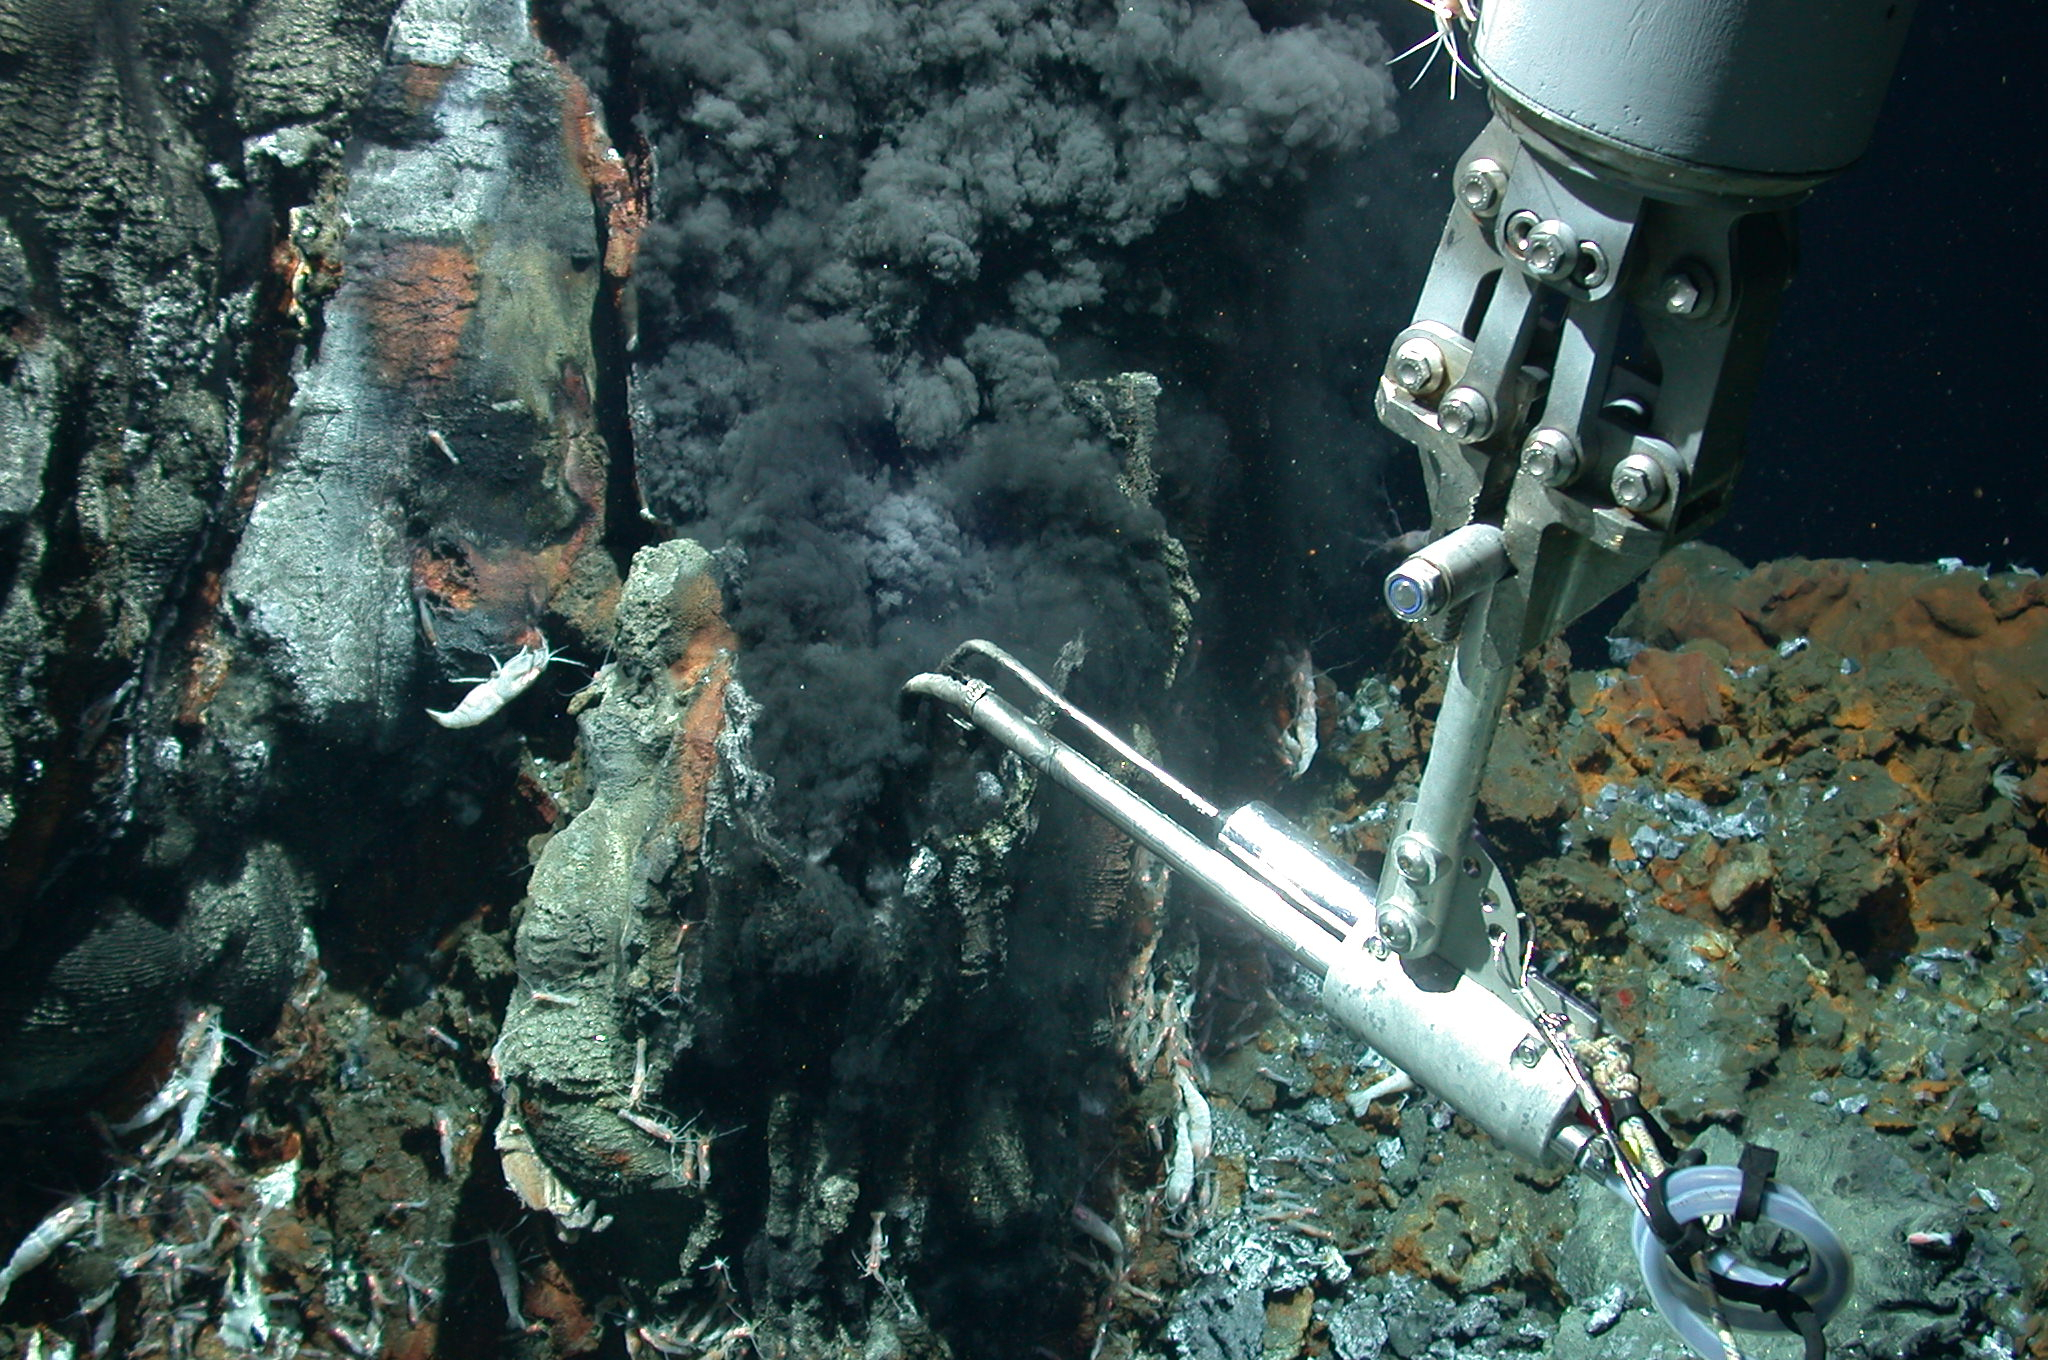
\includegraphics{Koschinsky_raw0.eps}}		  
%#.2x graphic -- 

\vspace{2.08mm}

\vspace{0.00mm}
\setlength{\parindent}{0.00mm}
\setlength{\leftskip}{0.00mm}
\setlength{\rightskip}{0.00mm}
\raggedright
Figure: Sampling of the hottest hydrothermal vent fluid found so far (407�C) at 5�S on the Mid-Atlantic Ridge during cruise M68/1. The fluid is taken with the KIPS fluid sampling system equipped with a temperature sensor. (Picture copyright: MARUM, Univ. Bremen)
\vspace{2.08mm}

\vspace{0.00mm}
\setlength{\parindent}{0.00mm}
\setlength{\leftskip}{0.00mm}
\setlength{\rightskip}{0.00mm}
\raggedright

\vspace{0.00mm}

\vspace{0.00mm}
\setlength{\parindent}{0.00mm}
\setlength{\leftskip}{0.00mm}
\setlength{\rightskip}{0.00mm}
\raggedright

\vspace{0.00mm}

\vspace{0.00mm}
\setlength{\parindent}{0.00mm}
\setlength{\leftskip}{0.00mm}
\setlength{\rightskip}{0.00mm}
\raggedright

\vspace{0.00mm}

\vspace{0.00mm}
\setlength{\parindent}{0.00mm}
\setlength{\leftskip}{0.00mm}
\setlength{\rightskip}{0.00mm}
\raggedright

\vspace{0.00mm}

\vspace{0.00mm}
\setlength{\parindent}{0.00mm}
\setlength{\leftskip}{0.00mm}
\setlength{\rightskip}{0.00mm}
\raggedright

\vspace{0.00mm}

\vspace{0.00mm}
\setlength{\parindent}{0.00mm}
\setlength{\leftskip}{0.00mm}
\setlength{\rightskip}{0.00mm}
\raggedright

\vspace{0.00mm}

\vspace{0.00mm}
\setlength{\parindent}{0.00mm}
\setlength{\leftskip}{0.00mm}
\setlength{\rightskip}{0.00mm}


\vspace{0.00mm}


\end{document}
